\documentclass[12pt]{jarticle}
\setlength{\columnsep}{3zw}


\usepackage[dvipdfmx]{graphicx}
\usepackage[hang,small,bf]{caption}
\usepackage[subrefformat=parens]{subcaption}
\captionsetup{compatibility=false}

\graphicspath{{./image/}}

\title{楽器演奏におけるテンポ加速現象の解明}

\author{奥屋 直己}

\usepackage[height=26cm,width=16cm]{geometry}

\begin{document}

\maketitle

\section{はじめに}
音楽の演奏において,テンポを一定に保ち続けることは最も重要なことの一つである.しかし,演奏者の意図にかかわらずにテンポ変化が生じることがあり,そのような場合の多くは,テンポが加速する方向に変化する.このような意図しないテンポ変化は,演奏者の間で「走る」という表現で共有され,だれもがよく経験する現象である.この「走る」現象は,事前に計画した表現の意識が弱まることや,合奏での演奏者間同期を妨げる要因となり,好ましくない現象とされている.この「走る」現象の原因として演奏者の間では,演奏者の心理的影響(不安や緊張,興奮など)が指摘されることが多い.しかし,いくつかの実験によると「走る」現象が起こりやすいテンポ,リズムパタンなどがあり,心理的影響以外によっても引き起こされることが報告されている.

Collyer ら\cite{Collyer}は,メトロノームと同期してレバーを押し,メトロノームが停止した後も同じテンポでレバー押しを継続する課題(同期継続課題:synchronization-continuation task)を用いた実験を報告している.彼は,27種類の目標テンポ条件(タッピング間隔として,175-825 msの範囲,テンポとして73-343 bpm)において同期継続課題を被験者に課し,テンポが遅くなりがちなテンポ帯と速くなりがちなテンポ帯があることを見出している.これによると,タッピング間隔が250-413 msおよび513-748 ms(80-117,145-240 bpm)の範囲でテンポが加速しやすく,それ以外の範囲では減速しやすかったという.さらに,永島ら \cite{Nagasima}はリズムや強弱といった実際の音楽演奏に含まれるリズムパタンでの同期継続課題を用いた実験を報告している.彼らは図\label{Nagasima}の12種類(aは統制条件)のリズムパタンにおいて,130 bpmのテンポで同期継続課題を被験者に課した.その結果,リズムパタンの異なるExpt.1では条件cおよびeで安定的にテンポが減速した.アクセントパタンが異なるExpt.2では条件bでテンポの加速,条件gでテンポの減速がみられ(条件c,dでも加速傾向がみられたが,被験者のばらつきが大きかった),リズムパタンや強弱パタンがテンポ維持に影響を及ぼすことがわかったという.
このように様々なテンポやリズムパタンで同期継続課題を行ってこられた.しかし,これらの実験の多くが演奏中に「走る」現象が起こりやすいテンポやリズムパタンを見つけることを目的としており,なぜ「走る」現象が起こるのかを検証した研究は少ない.

以上のことから,本実験では「走る」現象が起こる原因を解明するために,リズムパタンとアクセントパタンを伴うタッピングの同期継続課題に対して,タッピングする手の振り上げ幅がテンポ維持特性に与える影響を実験的に検討した.具体的には,被験者に対して5種類のリズムパタンをそれぞれ「何も指示しない場合」「手を大きく振り上げるよう指示した場合」「手を小さく振り上げるよう指示した場合」の3種類の指示で90秒間のタッピング同期継続課題を課し,タッピング中のタッピングの強さと手の振り上げ幅を計測し,解析した.

本論文の攻勢は以下の通りである.第2章では実験方法について述べ,第3章では結果およぼ考察を行う.第4章では,まとめを述べる.
\begin{figure}
  \centering
  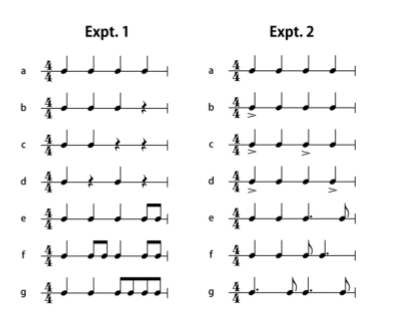
\includegraphics[width=10cm]{Nagasima.jpg}
  \caption{実験で用いたリズムパタン\cite{Nagasima}.}
  \label{Nagasima}
\end{figure}

\section{実験方法}
本実験では,手先を使ったタッピングによる同期継続課題を用いる.同期継続課題とは,初めはメトロノームと同期してリズムタッピングを行い,数秒後にメトロノームが消えた後もリズムタッピングを続けると言うものである.メトロノームのテンポは永島ら \cite{Nagasima}が行った実験同様120 bpm(時間間隔で500 ms)に設定した.被験者には5つのリズムパタン(図\ref{pattern})をそれぞれ「何も指示しない場合」「できるだけ大きく動かす」「できるだけ小さく動かす」の3つの指示でタッピングを行ってもらった.

\begin{figure}
  \centering
  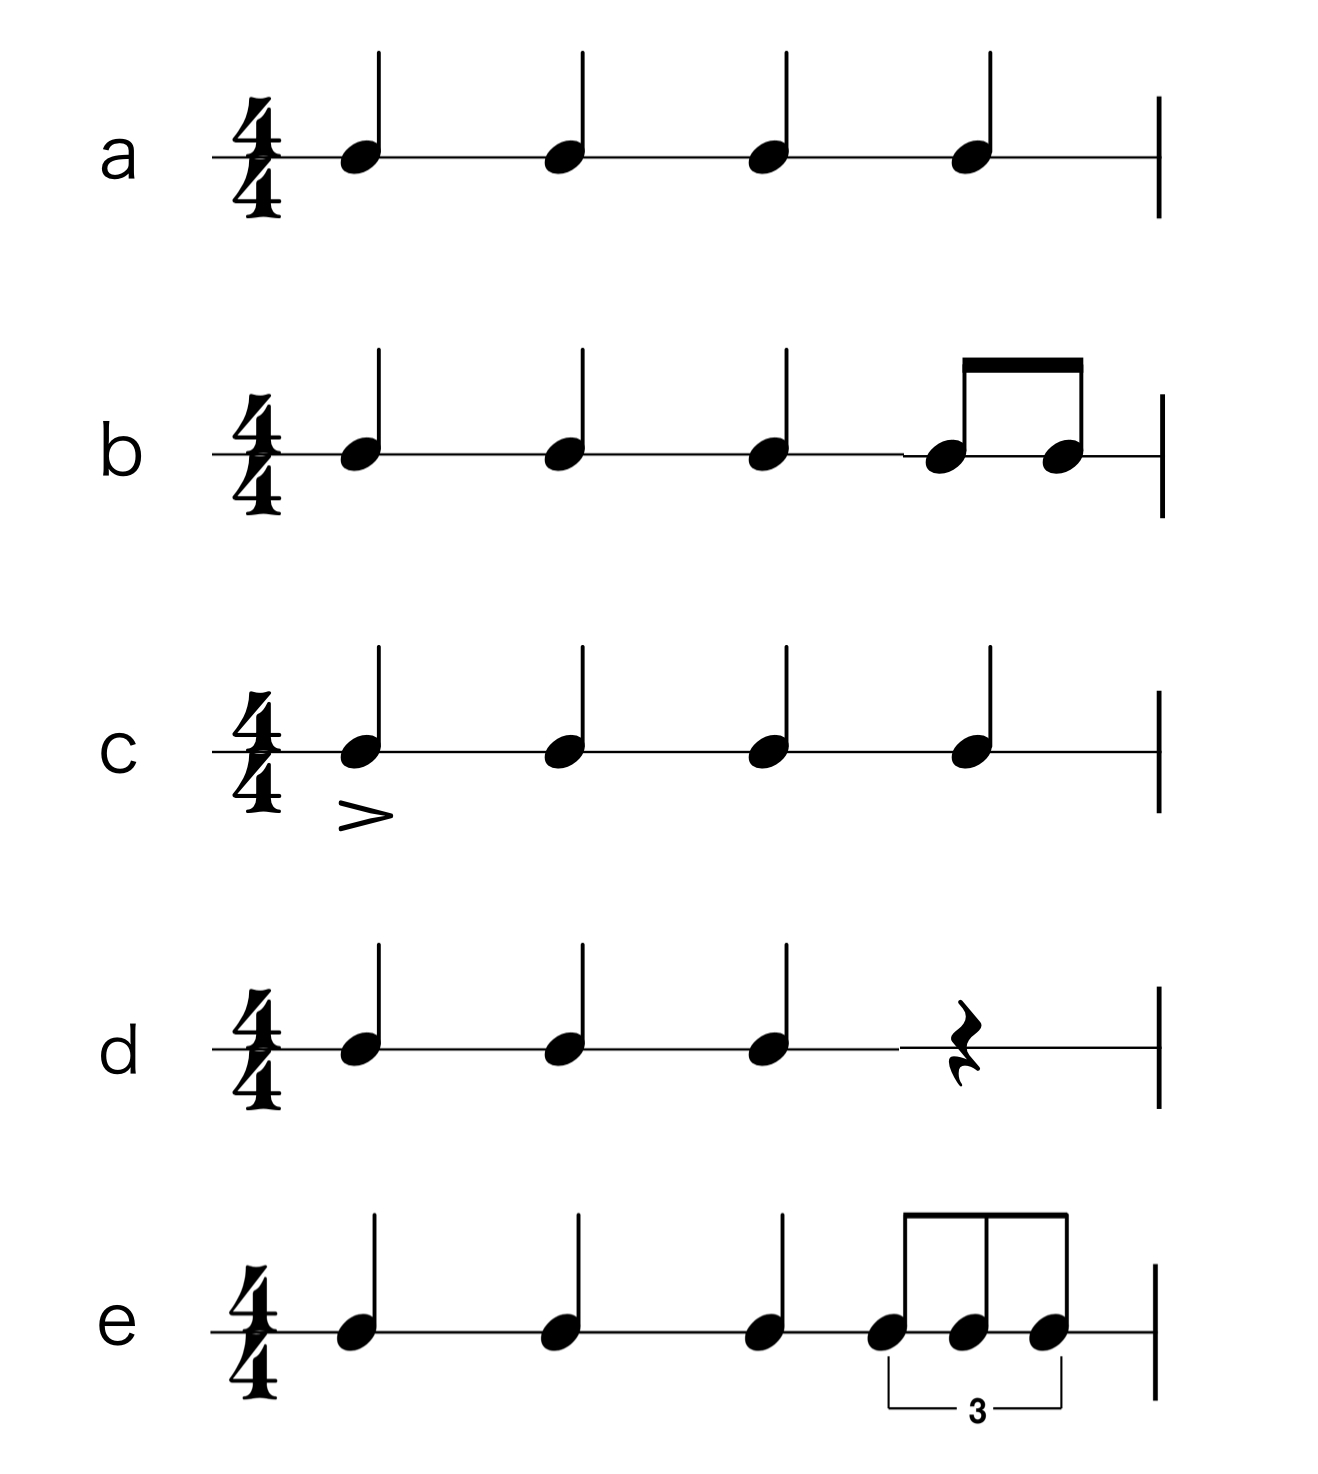
\includegraphics[width=7cm]{pattern.jpg}
  \caption{タッピングするリズムパタン.}
  \label{pattern}
\end{figure}  

\subsection{被験者}
本実験には10名(男性○,女性○)の被験者が参加し.楽器演奏経験の乏しい被験者では安定したリズムパタンの再生が困難である場合が多いため,本実験の被験者には何らかの楽器演奏経験,あるいはダンス経験がある被験者のみを対象に行った.被験者には謝礼として,図書カード1000円分を手渡した.

\subsection{装置}
被験者のタッピング動作の記録には,マイクロコンピュータ(Aruduino:Aruduino Uno)に圧力センサ(Interlink Electronics:FSR406)と赤外線距離センサ(STMicroelectronics:VL6180X)を組み合わせた装置を用いる(図\ref{device}).装置は上から圧力センサ,透明なアクリル板,赤外線距離センサの順に組み合わせた.また,装置内部の配線などが被験者に見えてしまうと被験者の意識が装置内部の配線に向いてしまわないように,ゴムシートをアクリル板上に貼り付けた.ただし,圧力センサ部分と赤外線距離センサの上部にはゴムシートを張り付けなかった.アクリル板が赤外線距離センサに及ぼす影響については,アクリル板がある場合とない場合で赤外線距離センサの値に違いがなかったことから赤外線距離センサがアクリル板に影響されないことを確認した.図\ref{distance_true}はアクリル板から一定の高さの物に対し,2秒間記録したときの実際の高さ(x軸:TRUE)と赤外線距離センサが示した値(y軸:REAL)をプロットしたグラフである.実際の高さに対して赤外線距離センサの示した値は$\pm{2}$ mmほどの誤差があるが15 cmあたりまで比例関係が成り立っている.15 cm以上のとき,センサの値は180 mmに収束している.しかし,被験者のタッピング中の手の高さは最大15 cmあたりまでだったので,赤外線距離センサが示した値を実際の距離のとして扱った.
Aruduinoでは圧力センサ,赤外線距離センサをサンプリングレート200\ Hz,100\ Hzで記録した.記録した値はシリアル通信(2000000 bps)を使い,PC上のprocessingにて作成したプログラムで受信し,csv形式で出力した.

\begin{figure}[htpb]
  \begin{minipage}{\hsize}
    \centering
    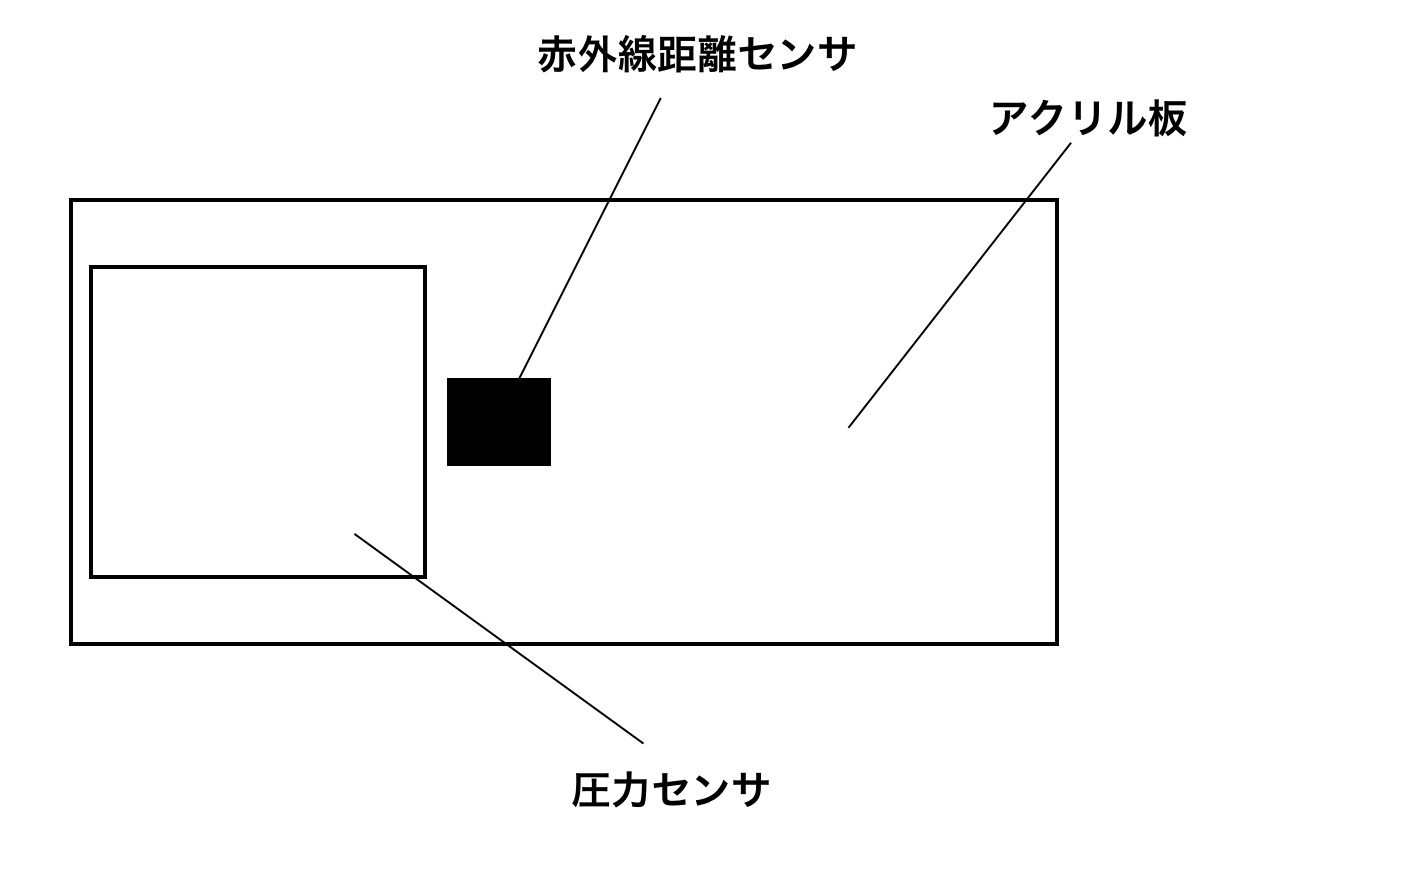
\includegraphics[width=7cm]{device_up.jpg}
    \subcaption{タッピング用の装置を上から見た図.}
    \label{device_up}
  \end{minipage}
  \begin{minipage}{\hsize}
    \centering
    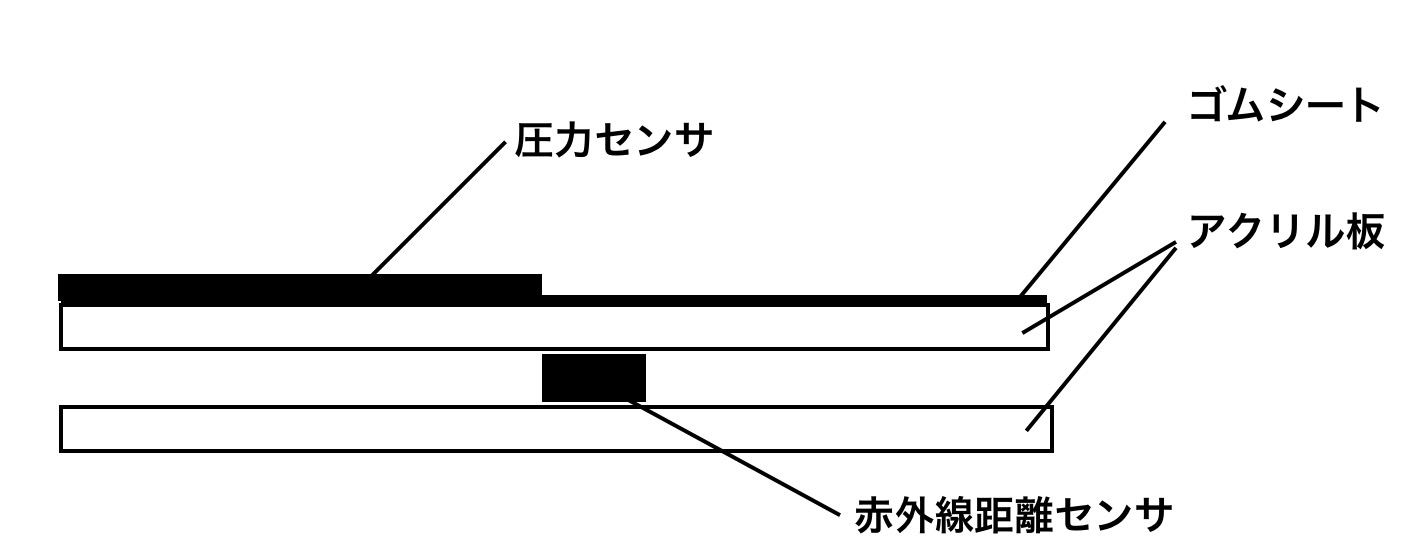
\includegraphics[width=7cm]{device_side.jpg}
    \subcaption{タッピング用の装置を横から見た図.}
    \label{device_side}
  \end{minipage}
  \caption{タッピング用装置.被験者には装置の配線などが見えないようゴムシートを用いて隠した.}
  \label{device}
\end{figure}

\begin{figure}
  \centering
  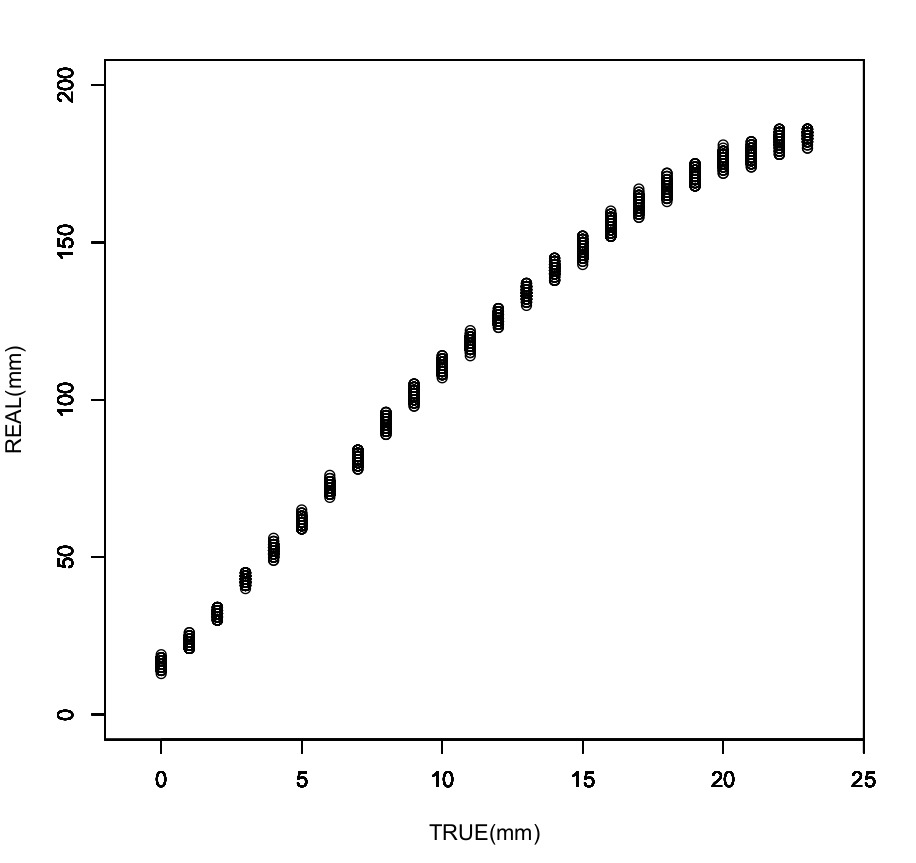
\includegraphics[width=7cm]{distance_true.jpg}
  \caption{実際の装置からの距離(x軸:TRUE(mm))と装置の値(y軸:REAL(mm)).}
  \label{distance_true}
\end{figure}

\subsection{同期継続課題中の被験者について}
被験者には図\ref{subject}のように椅子に座った状態で,机上の高さ9 cmの台に手首から肘方向に16 cmの区間を乗せ,手首から先を使ってタッピング装置をタッピングするように指示した.タッピングの際の手は図\ref{hand}のように親指以外の指を少し曲げ,親指は人差し指の第2関節あたりにつけるようにし,なるべく力を入れないように指示した.左右の手でタッピングが行いやすい方を被験者に選択してもらった.また,タッピングの際に距離センサの赤外線が指と指の間を通らないように親指以外の指をすべて覆うようにサージカルテープを巻いた.

\subsection{同期継続課題について}
本実験では,4分の4拍子で4小節の間(時間にして8秒間)メトロノームと同期して指定したリズムパタンでタッピングを行い,メトロノームが消えた後も同じリズムパタンで90秒間タッピングを行ってもらった.リズムパタンは図\ref{pattern}のa-eの順で行われ,それぞれで「何も指示をしない」「なるべく大きく動かす」「なるべく小さく動かす」の3つの指示で行ってもらった.ただし,指示の順はそれぞれのパタンで初めに「何も指示しない」を行い,2回目と3回目の「なるべく大きく動かす」「なるべく小さく動かす」の指示を被験者ごとに入れ替えた.


\begin{figure}
  \centering
  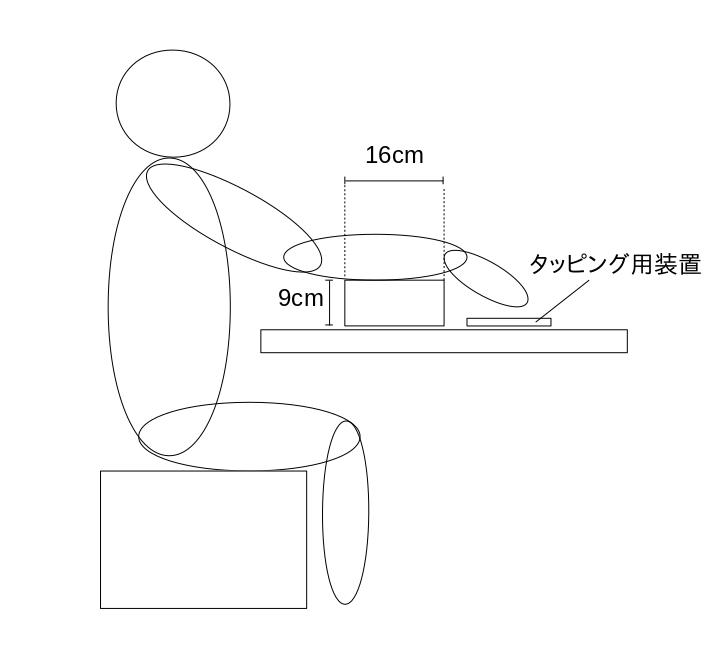
\includegraphics[width=7cm]{subject.jpg}
  \caption{被験者がタッピングする際の体勢.9 cmの台に腕を置き,手首から先を動かしタッピングを行う.}
  \label{subject}
\end{figure}
\begin{figure}[htpb]
  \begin{minipage}{\hsize}
    \centering
    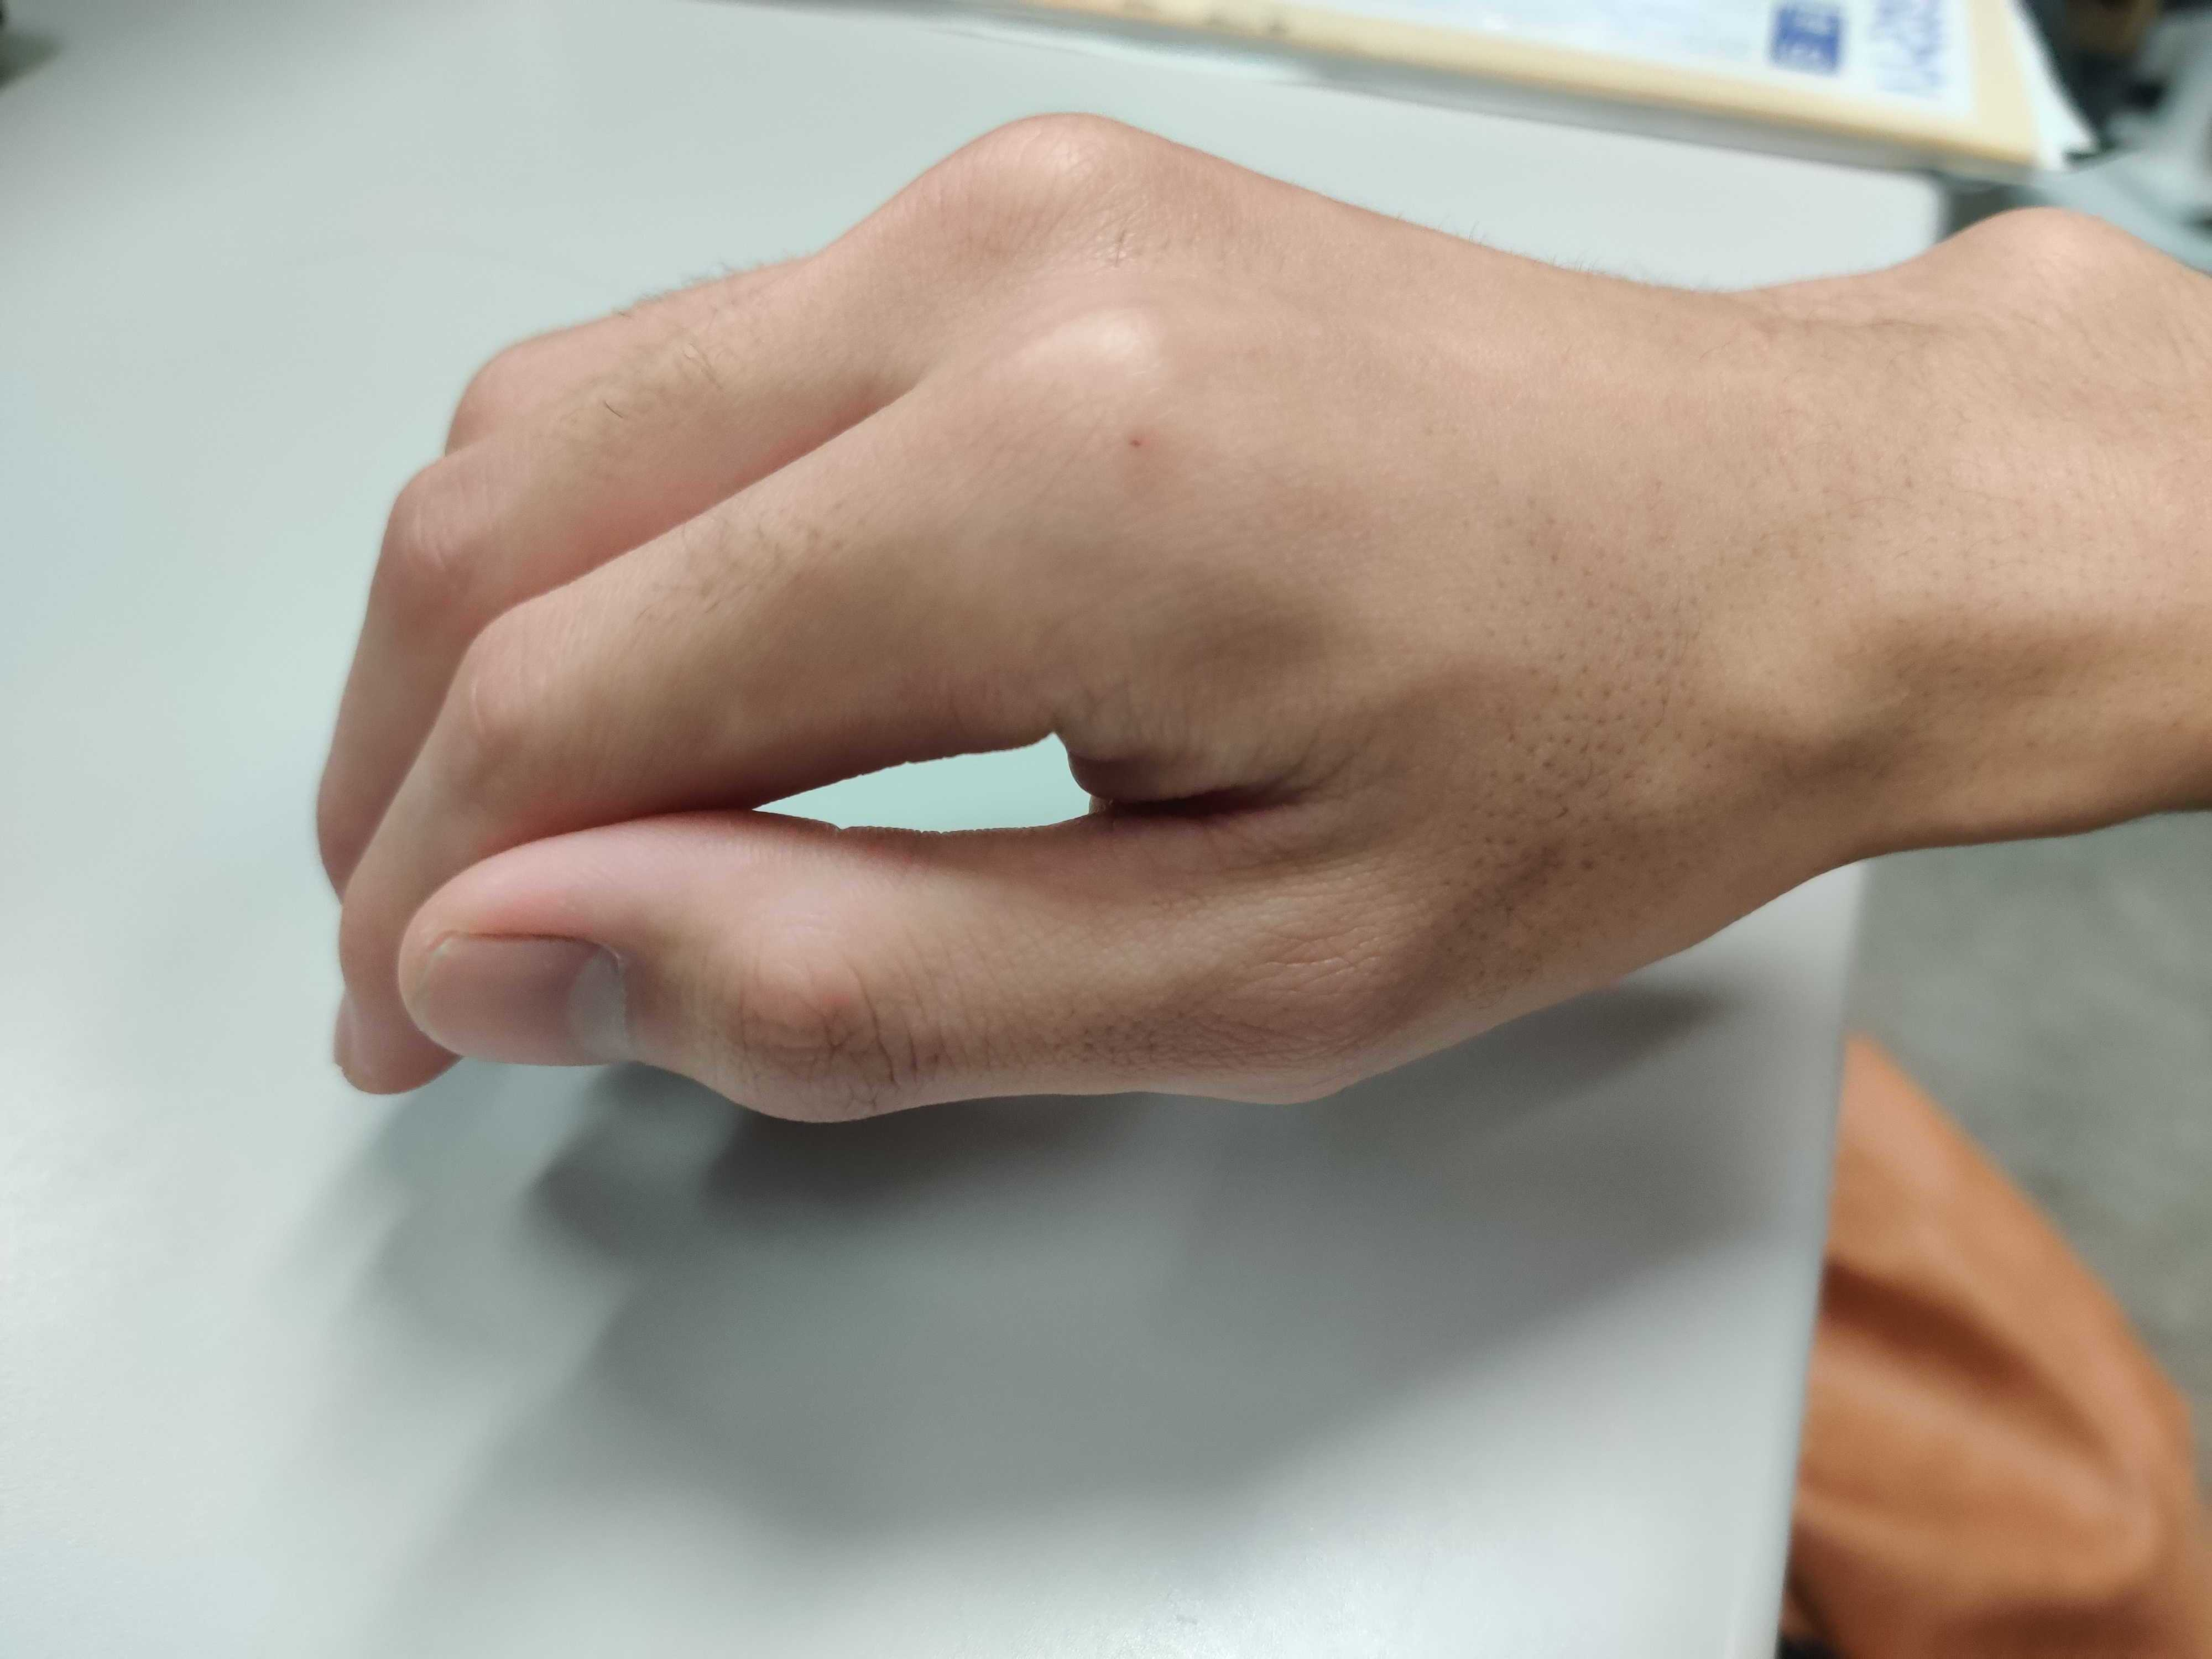
\includegraphics[width=7cm]{tapping_hand_1.jpg}
    \label{hand_1}
  \end{minipage}
  \begin{minipage}{\hsize}
    \centering
    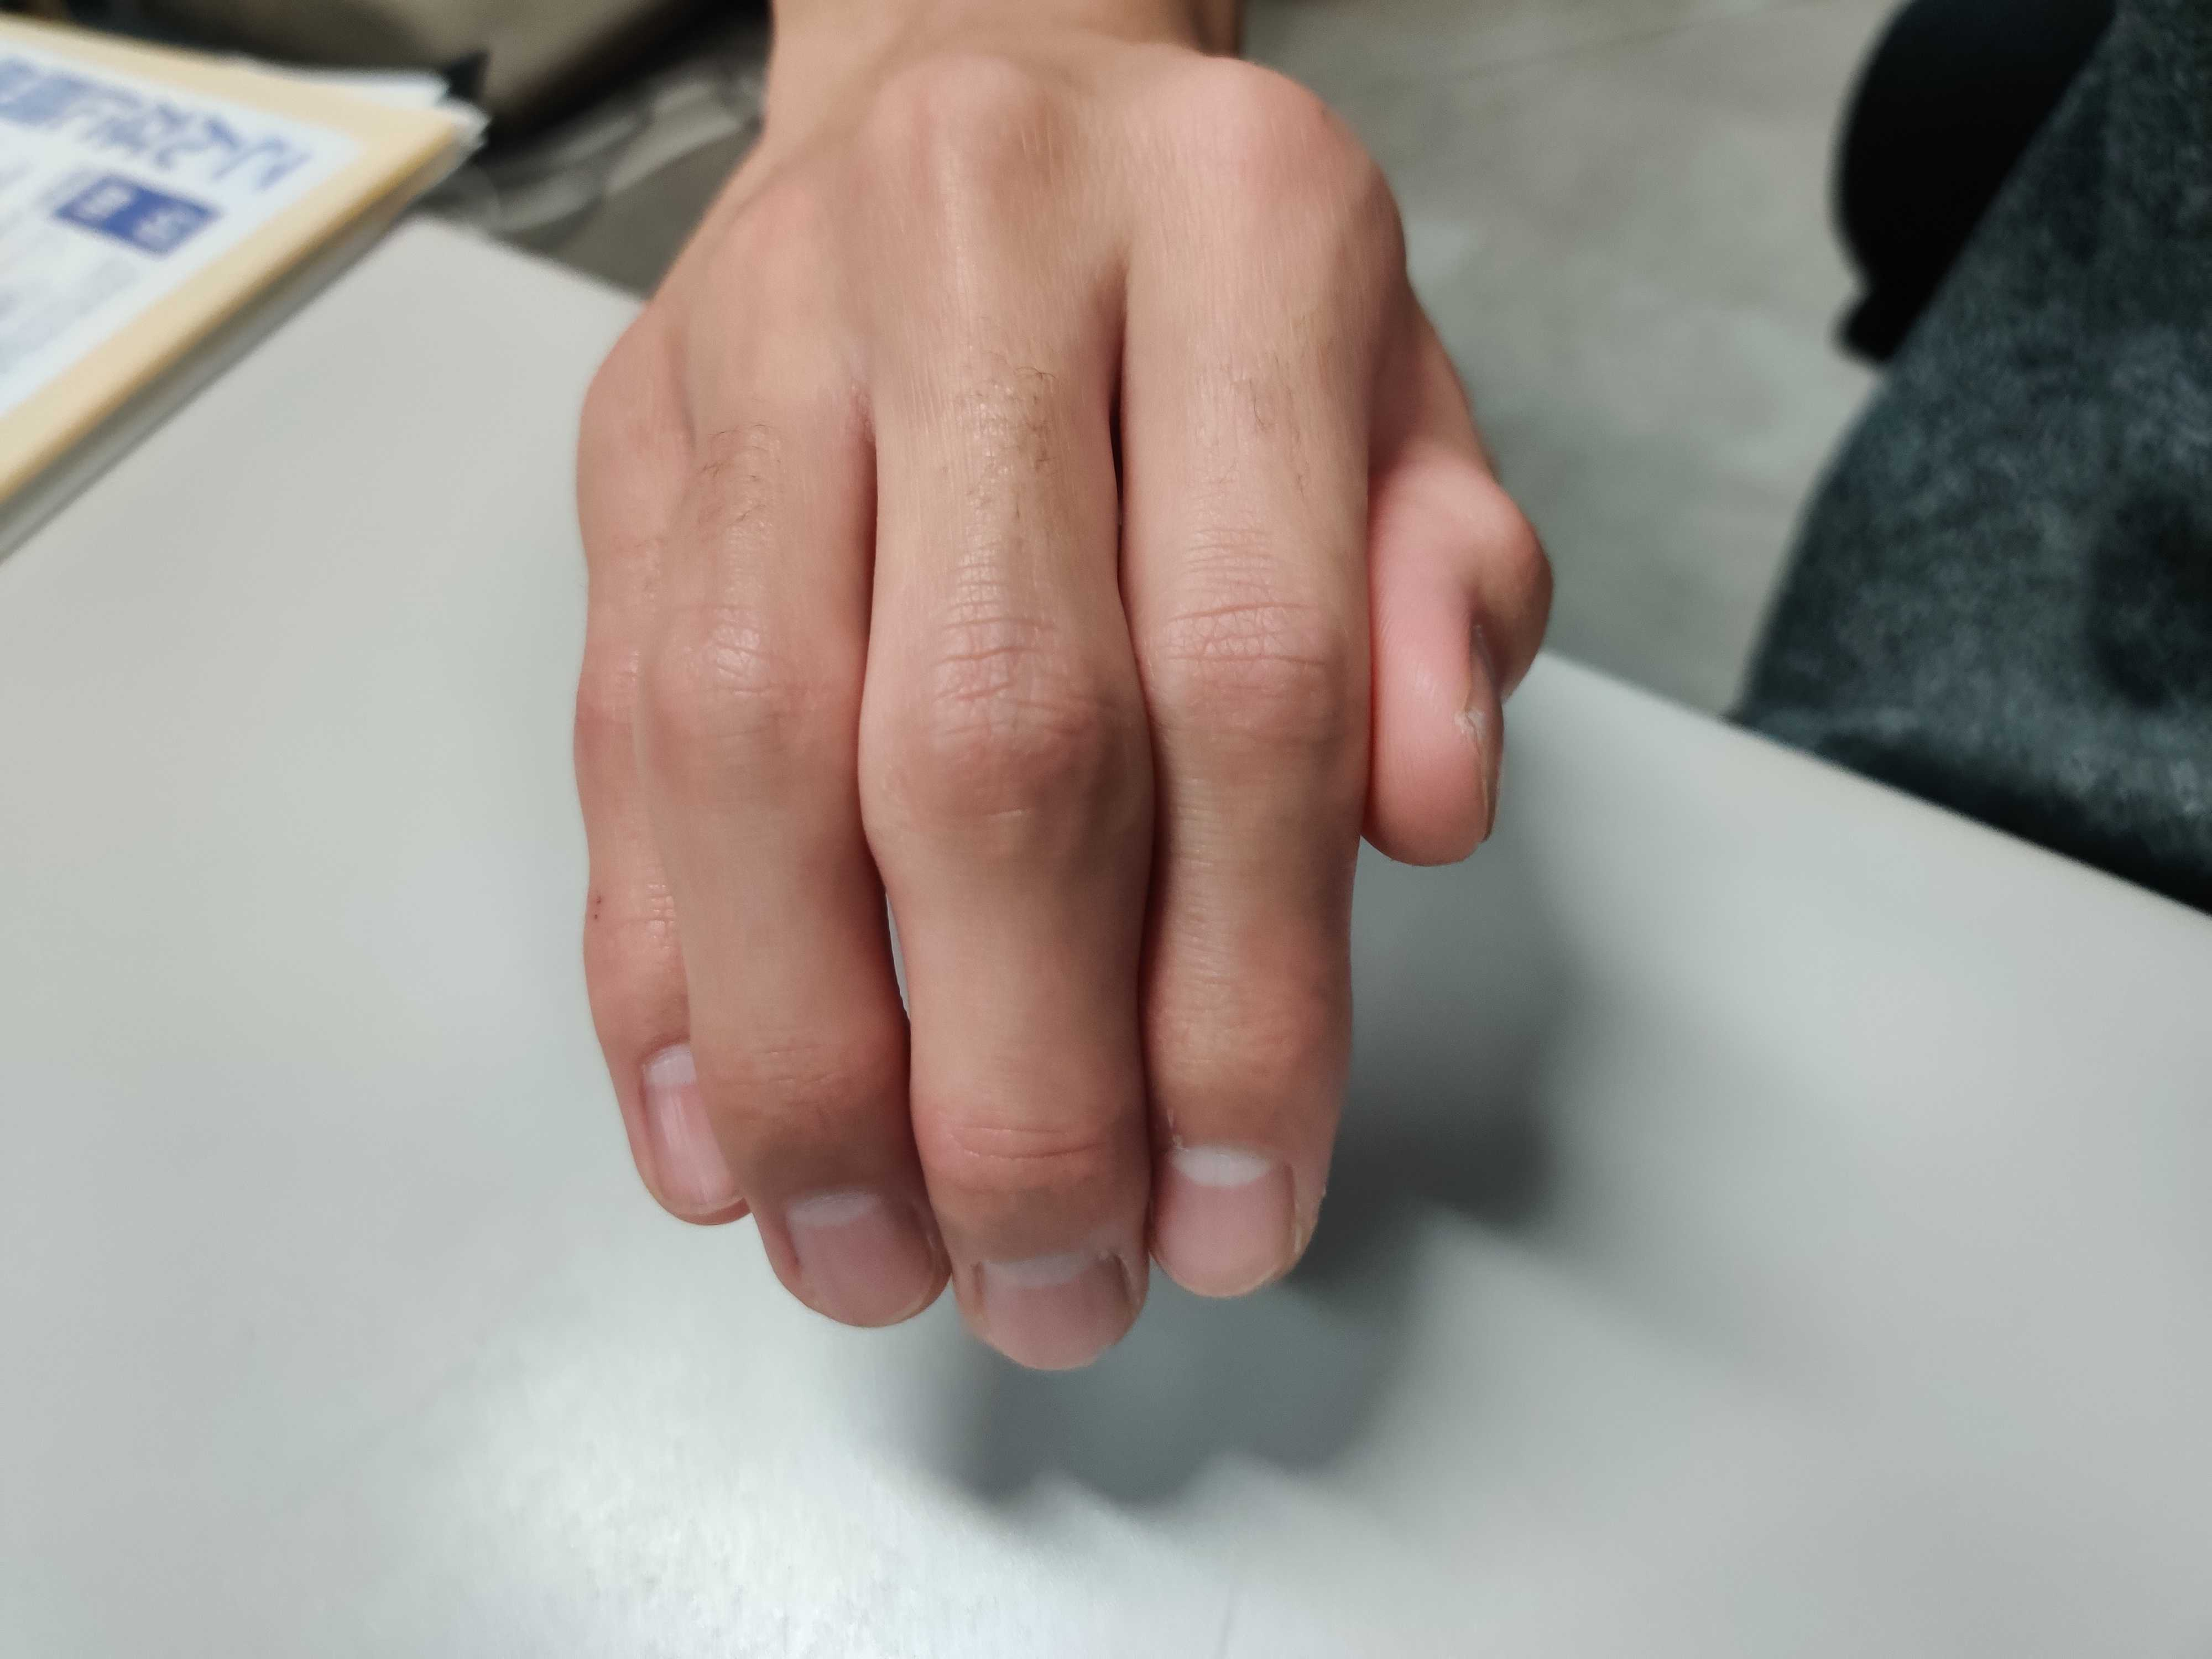
\includegraphics[width=7cm]{tapping_hand_2.jpg}
    \label{hand_2}
  \end{minipage}
  \caption{タッピング中の手の形}
  \label{hand}
\end{figure}
\subsection{条件}
本実験では,タッピング間隔が一定である統制条件と,2種類のリズムおよびアクセントパタンでタッピングを行う条件を設けた.条件aは統制条件,b,cはそれぞれ永島氏と坂口氏 \cite{Nagasima}の報告から,テンポ変化が起きなかったリズムパタンとテンポが安定的に加速したアクセントを含むリズムパタンである.

\subsection{手続き}
実験で使用するリズムに慣れるために,各リズムを使用した実験を行う前に,そのリズムで同期区間8小節,継続区間8小節の練習課題を課した.被験者がリズムパタンを理解し,タッピングできることを確認した後,同期区間 32拍分,継続区間 320拍分の本試験を行った.1試行に要した時間は2分弱である.したがって,実験全体で要した時間は,準備の時間も含めておよそ1時間だった.

\subsection{解析}
本実験の結果を統計的に検証するため,第2から第80までの各小節の小節長と第1小節の小節長との違いを順序尺度により検定した.

\bibliography{design}
\bibliographystyle{junsrt}

\end{document}
